
 				Vaadin\cite{vaadin} es un framework de desarrollo de SPA que permite escribir el código de dichas aplicaciones en Java o en cualquier otro lenguaje soportado por la JVM 1.6+. Esto permite la programación de la interfaz gráfica en lenguajes como Java 8, Scala o Groovy, por ejemplo.
 			
 		\vspace{5mm}
 		
 				Una de las características diferenciadores de Vaadin es que, contrario a las librerías y frameworks de JavaScript típicas, presenta una arquitectura centrada en el servidor, lo que implica que la mayoría de la lógica es ejecutada en los servidores remotos. Del lado del cliente, Vaadin está construido encima de Google Web Toolkit, con el que puede extenderse.
 	
 	\vspace{5mm}
 		
 				En este proyecto, Vaadin se encargara de realizar la comunicación entre el cliente y el servidor. De esta forma, será capaz de enviar y recibir datos, eventos y peticiones entre el componente Javascript (cliente) y el servidor.
 			
 			\vspace{5mm}
 			
	 			\begin{figure}[H]
	 				\centering
	 				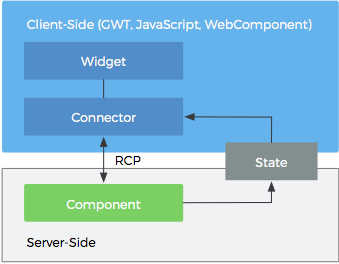
\includegraphics[scale=1.5]{schema.png}
	 				\caption{Esquema Cliente-Servidor}\label{fig:schema}
	 			\end{figure}